\section{How to Play}

\subsubsection*{Controls}
Controls are largely dependent on the platform you decide to play minesweeper on. The following are universal actions and the keybinds I tend to find associated with them when playing with mouse and keyboard.
\begin{itemize}
    \item \textbf{Start a new game}: Click the smiley face, F2 (also Spacebar for minesweeper.online)
    \item \textbf{Clear}: Left-Click
    \item \textbf{Flag/Unflag}: Right-Click
    \item \textbf{Chording}: Left+Right-Click, Middle-Click (also Left-Click for minesweeper.online)
\end{itemize}
Note: For some versions, right clicking will cycle through a flag, a ? question mark, and an unmarked square. If able, I recommend turning off ``Marks (?)" in the settings, as question marks don't serve too much utility while playing.\\


\subsubsection*{Clearing Squares}
Left-clicking on a square is a commitment. You are declaring, ``I swear on my life that there is no mine on this square." Should you left-click on a square containing a mine.\\

\textbf{Clearing}\index{Clear} an unknown square checks the value of the square. Four things can happen when you clear a square:
\begin{enumerate}
    \item There is no mine in the square, and a number appears. This number indicates the number of mines in the eight neighboring squares (or less if the square is on an edge).
    \item There is no mine in the square, and many numbers appear. This is called an \textbf{opening}\index{Opening}. An opening occurs when there are no mines in the square you click, as well as the squares neighboring the square you click. This is an effective ``0" number, but games typically leave the square blank, and automatically clears all the squares around the zeros recursively until no more squares can be cleared.
    \item You click a mine. You are dead.
    \item You've cleared the last square that's not a mine. You've won the game
\end{enumerate}
\begin{figure}[h]
    \centering
    \begin{subfigure}[t]{0.2\textwidth}
        \centering
        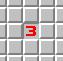
\includegraphics[width=0.8\linewidth]{figures/2.1/single}
        \caption{Single number}
    \end{subfigure}
    \begin{subfigure}[t]{0.2\textwidth}
        \centering
        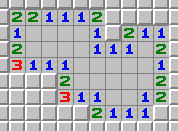
\includegraphics[width=0.8\linewidth]{figures/2.1/opening}
        \caption{Opening}
    \end{subfigure}
    \begin{subfigure}[t]{0.2\textwidth}
        \centering
        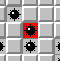
\includegraphics[width=0.8\linewidth]{figures/2.1/mine}
        \caption{Mine}
    \end{subfigure}
    \begin{subfigure}[t]{0.2\textwidth}
        \centering
        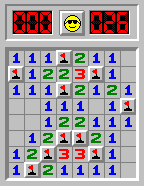
\includegraphics[width=0.8\linewidth]{figures/2.1/win}
        \caption{Win (Note the sunglasses on the smiley face}
    \end{subfigure}
    \caption{The four possible scenarios when clearing a square}
\end{figure}


\subsubsection*{The First Click}
The game starts when you clear the first square. The first left-click you make is guaranteed to never be a mine. Leaving the details for future sections (Section \ref{sec:simple_guessing}), basic rule of thumb is to \textbf{choose a corner for your first click}. The idea is to hope for an opening on your first click that will minimize the amount of needed guessing. Hand waving a lot, corners are a good choice because it only has 3 neighbors, giving it the high odd of having no neighboring mines, leading to an opening. If the first corner does not lead to a sufficient opening, clicking on other corners is also an okay idea (more on this later).\\


\subsubsection*{Use Flags to Mark Where You Think Mines Are}
\textbf{Flags}\index{Flag} can be placed on the grid by right-clicking a square. This will decrement the mine counter. Flags can still be placed on squares without a mine, and this will still decrease the mine counter. Flags do NOT verify that a mine is at a given square. They are simply a useful tool the player can use to mark possible mine locations.\\

Flagging is more than just a visual aid. They can be used for chording (discussed below), minecounting (Section 3.4), and for preventing possible misclicks onto the mine. For beginners and anyone not playing for speed, I highly recommend to \textbf{place a flag at every location you know there is a mine}.\\

Do note that there exists a ``No Flag" playstyle where players intentionally play without flags. This can improve speed in some cases since you are not using extraneous clicks to flag obvious mines. In section 5, we'll find that a hybrid approach where only some mines are flagged may actually be the fastest strategy. In my opinion, for higher difficulties expert and above, not flagging at all is psychotic, but if this is you, you do you.\\


\subsubsection*{Chording}
\textbf{Chording}\index{Chording} is a technique where you click a number with the number's number of flags adjacent to it (we'll call this a \textbf{chordable} number). This clears all the squares around the number you click (and if a surrounding square is an opening, a recursive clearing is performed).\\

Chording can be normally be performed with either a middle-click, or by pressing left and right-click at the same time. As chording typically follows placing a flag, you can keep holding the right-click from placing the flag, and left-click the fulfilled number next to the flag to chord. However, when the platform allows, sometimes just left-clicking the fulfilled number will also chord.\\

If used correctly, chording can greatly reduce the number of clicks you use. Like flagging, chording all the time is usually not optimal for speed. However, advanced players can use chording to speed up clears. For beginners, chording is hardly necessary to know, but I personally used chording a lot when learning. Chording reduces the number of raw left-clicks you perform on the unknown squares, reducing possible misclick encouters.\\